%% Copyright (C) 2012 Minh Van Nguyen <mvngu.name@gmail.com>
%% This work is licensed under a the GNU Free Documentation License version
%% 1.3.  For the full terms of the license, see
%% http://www.gnu.org/licenses/fdl.html

\documentclass{beamer}

\usepackage{mystyle}


%%%%%%%%%%%%%%%%%%%%%%%%%%%%%%%%%%%%%%%%%%%%%%%%%%%%%%%%%%%%%%%%%%%%%%%%%%%

\title[Evolution of communities]{
  Community evolution in a scientific collaboration network
}
\institute{
  \large $^1$University of Melbourne, $^2$CSIRO
}
\author[Nguyen~et~al.]{
  Minh Van Nguyen,$^1$ Michael Kirley,$^1$ and \\
  Rodolfo Garc\'ia-Flores$^2$
}
%% uncomment the following line for the current date
\date{\small \today}
%% \date{}


%%%%%%%%%%%%%%%%%%%%%%%%%%%%%%%%%%%%%%%%%%%%%%%%%%%%%%%%%%%%%%%%%%%%%%%%%%%

\begin{document}

\frame{\titlepage}


%%%%%%%%%%%%%%%%%%%%%%%%%%%%%%%%%%%%%%%%%%%%%%%%%%%%%%%%%%%%%%%%%%%%%%%%%%%

%% Uncomment this section for the table of contents.
%% \frame{
%%   \frametitle{Contents}
%%   \tableofcontents
%% }


%%%%%%%%%%%%%%%%%%%%%%%%%%%%%%%%%%%%%%%%%%%%%%%%%%%%%%%%%%%%%%%%%%%%%%%%%%%

\section{Introduction}
%%
\frame{
  \frametitle{Introduction}
  %%
  \begin{itemize}
  \item The presence of communities in social networks is intuitive.
    %% Think of members of a social club such as a sports club, a
    %% professional association such as the ACM, the developers of a
    %% software project, or online communities such as Facebook
    %% groups.  The concept of communities can also be transferred to
    %% other types of networks.  In a financial or economic network, a
    %% community might be a group of organizations that trade more
    %% amongst themselves than with other organizations.  In a
    %% software network, a community might be a group of functions or
    %% modules that invoke each other more often than other functions
    %% or modules in a software package.
  \end{itemize}

  \begin{figure}[!bp]
  \centering
  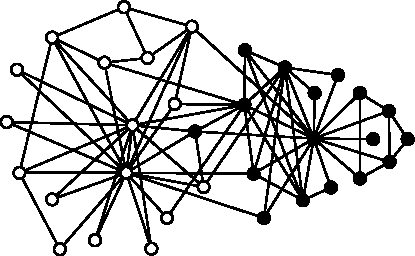
\includegraphics{image/Zachary-karate-club-community}
  \caption{Two communities in a karate club~\cite{Zachary1977}.}
  \end{figure}
}


%%%%%%%%%%%%%%%%%%%%%%%%%%%%%%%%%%%%%%%%%%%%%%%%%%%%%%%%%%%%%%%%%%%%%%%%%%%

\section{Motivation and aim}
%%
\frame{
  \frametitle{Motivation and aim}
  %%
  \begin{itemize}
  \item Uncover principles of community evolution.
    \begin{itemize}
    \item Understand how a blog network evolve~\cite{LinEtAl2008}
    \item Discover calling patterns \& customer churns in a mobile
      phone network~\cite{GreeneEtAl2010,PallaEtAl2007}
    \item Map out the long-term collaboration among groups of
      researchers~\cite{PallaEtAl2007}
    \end{itemize}

  \item How does community size affect the evolution of communities?
    %% The above general question can be answered along two separate
    %% lines.  One is to focus on the scaling characteristic of
    %% community size and any implication that this has for the
    %% long-term statistical properties of communities.  Another is to
    %% focus on any effects that the minimum community size has on
    %% events in the history of communities.
    \begin{itemize}
    \item What is the scaling characteristic of community size and the
      implication for community evolution?
      %% This relates to the long-term behaviour of the distribution
      %% of community size.

    \item How does the minimum size of communities affect the
      life-cycle of communities?
      %% This is about exploring the relationship between minimum
      %% community size and events in the history of communities.

    %% \item To what extent can the minimum community size be used to
    %%   filter out inactive communities?
    \end{itemize}
  \end{itemize}
}


%%%%%%%%%%%%%%%%%%%%%%%%%%%%%%%%%%%%%%%%%%%%%%%%%%%%%%%%%%%%%%%%%%%%%%%%%%%

\section{Background}

\frame{
  \frametitle{Background}
  %%
  \begin{itemize}
  \item Communities evolve according to a
    life-cycle~\cite{GreeneEtAl2010,PallaEtAl2007}:
    \begin{itemize}
    \item birth and death

    \item expand and contract

    \item merge and split
    \end{itemize}
  \end{itemize}

  \begin{figure}
  \centering
  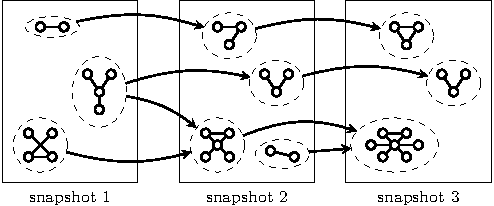
\includegraphics{image/match}
  \caption{The evolution of communities in terms of a life-cycle model.}
  \end{figure}
}


%%%%%%%%%%%%%%%%%%%%%%%%%%%%%%%%%%%%%%%%%%%%%%%%%%%%%%%%%%%%%%%%%%%%%%%%%%%

\bibliographystyle{bibliography.bst}
\bibliography{bibliography}

\end{document}
